\chapter{Project Design}

This chapter details the design and implementation of the models and algorithms used in this study. The goal is to simulate the spread of infectious diseases on different network structures and apply source detection algorithms to identify the origins of the infection. The design choices, methodologies, and tools used in this study are discussed comprehensively.

\section{Model Structures and Algorithm Implementation}

\subsection{Grid-based models}

The spread of disease in grid-based models is simulated by allowing the infection to propagate from one node to its neighboring nodes. The infection probabilities on neighbors in a grid-based model were discussed in detail in the Mathematical Modeling chapter along with the interaction rules in Section \ref{section:infection_probabilities}.

The structure of the grid-based model and the importance of boundary conditions were previously outlined in Section \ref{section:boundary_conditions}. To summarize, the boundaries of the grid significantly affect the spread dynamics. Fixed boundaries can limit the spread, while periodic boundaries simulate an infinite plane by wrapping around edges, allowing the infection to propagate without edge effects.

\subsubsection{Equilibrium State in Grid-Based Models}
An equilibrium state in a grid-based model is reached when the number of individuals in each state (susceptible, infected, recovered) stabilizes and no longer changes significantly over time. This state indicates a balance between the rates of infection, recovery, and return to susceptibility. Understanding the equilibrium state helps in predicting the long-term behavior of the disease spread and in designing effective intervention strategies.

\begin{figure}[H]
    \centering
    \includegraphics[width=0.9\textwidth]{equilibrium_state.png}
    \caption{SIRS Model Dynamics and Equilibrium State}
    \label{fig:equilibrium_state}
\end{figure}

\noindent
Figure \ref{fig:equilibrium_state} shows the dynamics of the SIRS model reaching an equilibrium state. Initially, the number of susceptible individuals (blue) decreases as the infection spreads, while the number of infected (red) and recovered (green) individuals increase. Over time, the system stabilizes, and the number of individuals in each state remains constant, indicating that the model has reached an equilibrium.

\subsubsection{Impact of Initial Infection Sources}
The initial number and location of infected nodes significantly impact the disease spread dynamics. Multiple initial infection sources can lead to a rapid spread and a higher initial peak of infected individuals, as the infection can propagate from several points simultaneously. Conversely, a single initial infection source typically results in a slower spread and a delayed peak.

\begin{figure}[H]
    \centering
    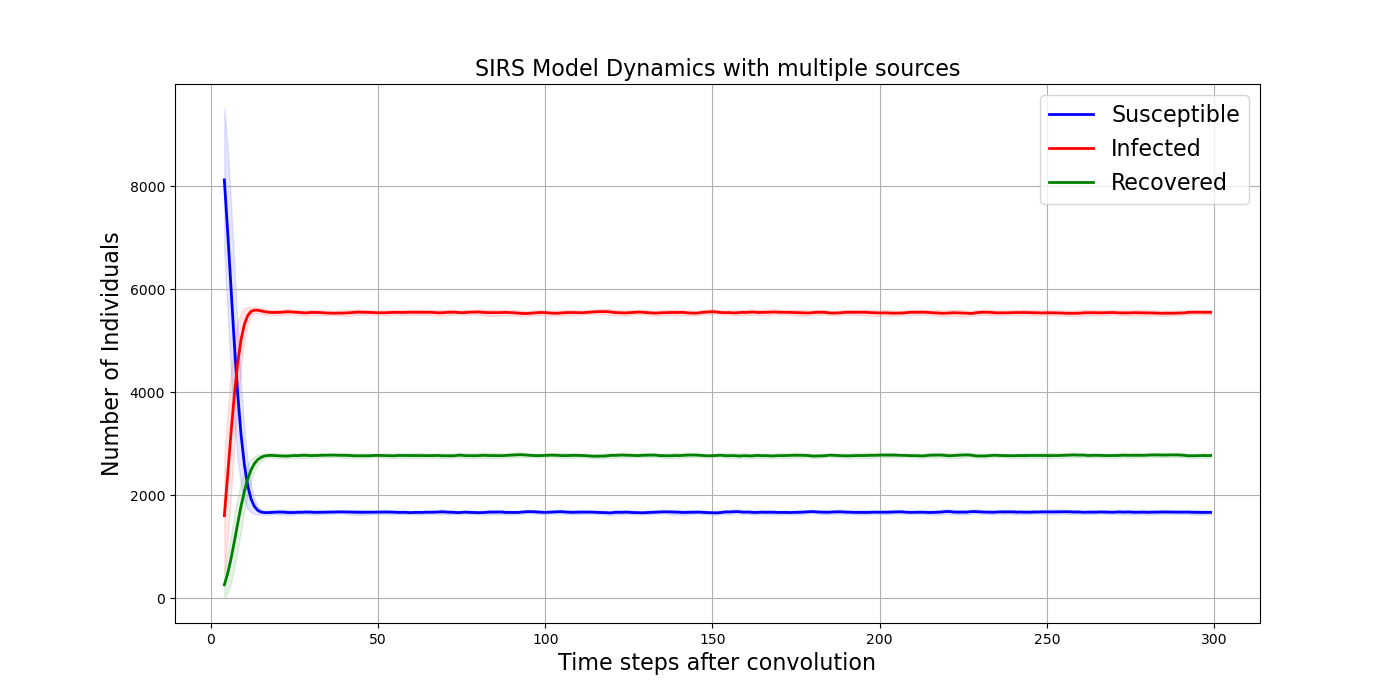
\includegraphics[width=0.49\textwidth]{multiple_sources.png}
    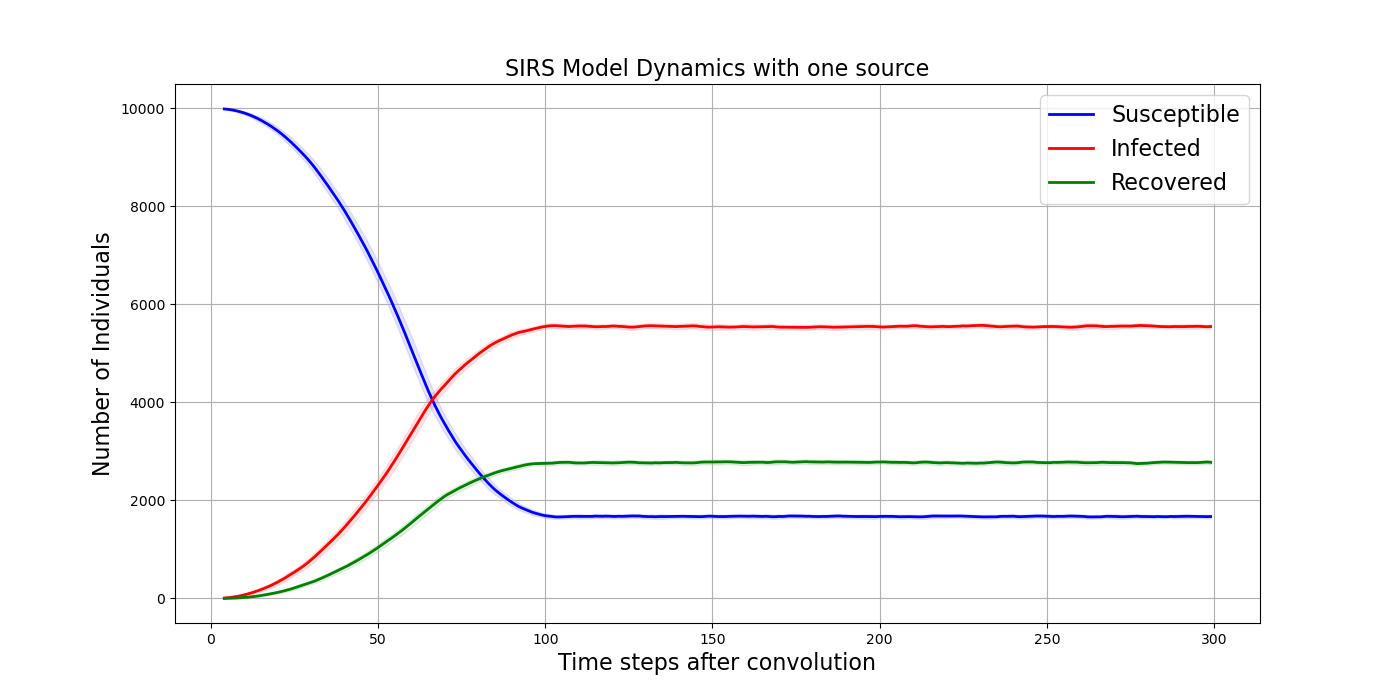
\includegraphics[width=0.49\textwidth]{one_source.png}
    \caption{Impact of Initial Infection Sources on Disease Spread}
    \label{fig:infection_sources_impact}
\end{figure}

\noindent
Figure \ref{fig:infection_sources_impact} illustrates the difference in disease spread dynamics between multiple and single initial infection sources. In the left panel, with multiple sources, the number of infected nodes rises sharply and then stabilizes as the disease quickly reaches an equilibrium. In the right panel, with a single source, the infection spreads more slowly, taking longer to reach the peak and stabilize.

By analyzing these dynamics, we can better understand how initial conditions affect the spread and control of infectious diseases in grid-based models. This understanding is essential for designing effective intervention strategies and predicting the outcomes of different epidemic scenarios.

\subsubsection{Comprehensive Insight into Grid-Based Models}
Grid-based models offer a controlled environment to study the spread of infectious diseases. By manipulating parameters such as infection probability, recovery rate, and initial infection sources, researchers can gain insights into the disease dynamics and the effectiveness of various intervention strategies. These models also provide a basis for comparing different algorithms for infection source detection, as discussed in the subsequent sections of this chapter.

\subsubsection{Source Detection Algorithms}
For source detection within the grid-based model, we implemented three primary algorithms: Jordan Center Identification using Breadth-First Search (BFS), Euclidean Distance Minimization, and Center of Mass Identification. These algorithms were evaluated based on their accuracy, complexity, and ability to handle boundary conditions.

\paragraph{Accuracy:}
The accuracy of each algorithm was measured by its ability to correctly identify the infection source within the grid. This was quantified by running multiple simulations (400 different grids each step) and recording the percentage of times the algorithm correctly identified the actual source. Higher accuracy indicates a more reliable algorithm for source detection.

\paragraph{Complexity:}
Complexity was evaluated based on the computational resources required by each algorithm, particularly focusing on time complexity. The Jordan Center Identification algorithm, using BFS, typically has a higher time complexity due to the exhaustive search required to compute the centrality scores for all candidate nodes. In contrast, the Center of Mass algorithm is computationally simpler as it only involves calculating the mean position of the external boundary nodes.

\paragraph{Boundary Handling:}
Boundary handling refers to the algorithm's ability to effectively manage the edges of the grid, where interactions may be limited or different from the interior. Algorithms that consider wrap-around boundaries or effectively account for fixed boundaries were rated higher in this metric. The performance in boundary handling was assessed by comparing the accuracy of each algorithm in grids with different boundary conditions (fixed and wrap-around).\\

The \textbf{Jordan Center algorithm} employs a Breadth-First Search (BFS) approach to identify the central node that minimizes the maximum distance to all other nodes. This method calculates the centrality score for each candidate node, selecting the node with the highest score as the source. The detailed implementation of this algorithm is presented in the Implementation chapter.

The next figures illustrate the performance of the Jordan Center algorithm in different grid configurations. The titles of the figures, such as "source\_recovery\_30\_70\_fixed\_grid," indicate that the true source node used in the algorithm is located at (30, 70) and that the grid has fixed boundaries. These images represent the results of running the source location algorithm on 400 different grids at each time step, with each grid being a 100x100 grid.

\begin{figure}[H]
\centering
\includegraphics[width=0.49\textwidth]{source_recovery_30_70_Fixed_Grid.png}
\includegraphics[width=0.49\textwidth]{source_recovery_30_70_Wrap_Around_Grid.png}
\caption{Source Recovery at (30, 70) with Jordan Center Algorithm on Fixed Grid (Left) and Wrap-Around Grid (Right)}
\label{handling_boundaries_jordan_center}
\end{figure}

Figure \ref{handling_boundaries_jordan_center} shows the performance of the Jordan Center algorithm in both fixed boundary and wrap-around grid configurations. In the fixed boundary grid (left), the accuracy of source recovery decreases significantly as the infection reaches the boundaries. This is because edge nodes have fewer neighbors, which skews the centrality calculations, leading to less accurate source detection. In contrast, the wrap-around grid configuration (right) maintains high accuracy due to consistent node behavior across the grid. The wrap-around boundaries eliminate the edge effects seen in fixed boundary grids, allowing for more accurate centrality measurements and, consequently, more precise source detection.

\begin{figure}[H]
\centering
\includegraphics[width=0.9\textwidth]{source_recovery_48_51.png}
\caption{Source Recovery (48, 51) with Jordan Center Algorithm}
\label{source_recovery_central_node_jordan_center}
\end{figure}

Figure \ref{source_recovery_central_node_jordan_center} demonstrates the high effectiveness of the Jordan Center algorithm when detecting the source at central nodes. The symmetric conditions in the center of the grid favor accurate source detection due to the uniform connectivity of nodes.

The \textbf{Jordan Center algorithm} performs exceptionally well in wrap-around grid configurations due to the consistent node behavior across the grid. This consistency allows for accurate centrality measurements, resulting in high source recovery accuracy. However, in fixed boundary grids, the algorithm's performance deteriorates as the infection reaches the boundaries. This analysis provides critical insights into selecting and adapting source detection algorithms based on the grid configuration and boundary conditions in epidemiological models.\\

We then explored the \textbf{Center of Mass Algorithm} for source detection. The Center of Mass algorithm calculates the mean position of all infected nodes and designates this point as the source of the infection. While this method is computationally efficient, it has limitations in terms of accuracy, particularly near the boundaries of the grid.

Initially, we applied the Center of Mass algorithm to detect the source node using the regular method. The results are depicted in Figure \ref{source_recovery_48_51_Center_of_Mass}, which shows a poor recovery of the source node.

\begin{figure}[H]
\centering
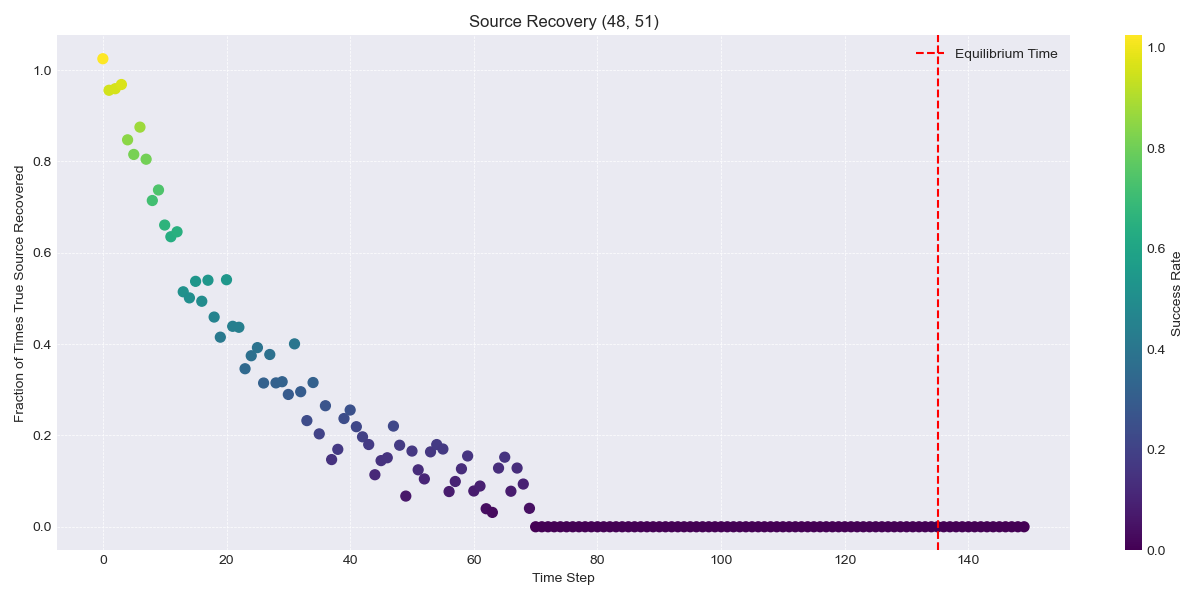
\includegraphics[width=0.9\textwidth]{source_recovery_48_51_Center_of_Mass.png}
\caption{Source Recovery (48, 51) with Center of Mass Algorithm}
\label{source_recovery_48_51_Center_of_Mass}
\end{figure}

Upon analyzing the distance error between the true source node and the recovered one, we observed that the error distance was usually small, especially in the initial stages of the infection spread. To better understand this, we plotted the distance error between the predicted source and the true source over time, as depicted in Figure \ref{Distance_Error_True_Predicted_Source_Center_Mass}. This analysis shows that the distance error remains relatively small in the initial stages of infection spread, justifying the one-node error margin approximation.

\begin{figure}[H]
\centering
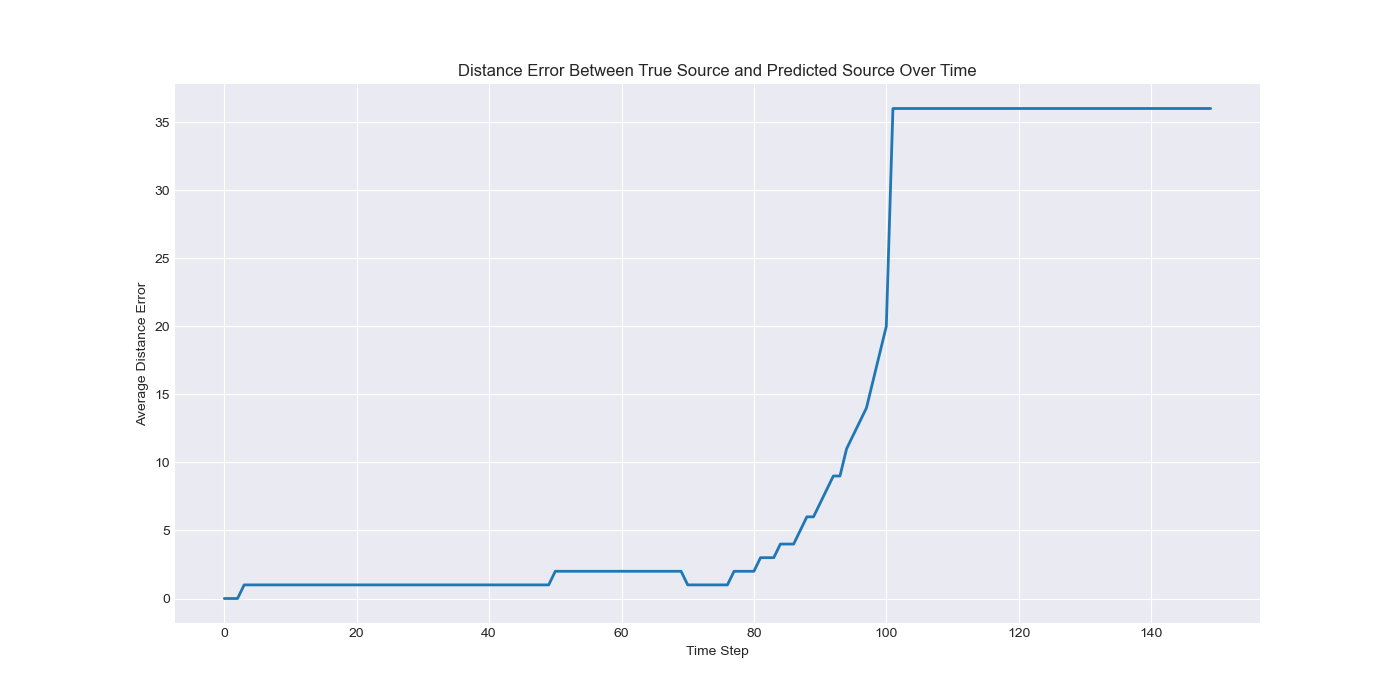
\includegraphics[width=0.9\textwidth]{Distance_Error_True_Predicted_Source_Center_Mass.png}
\caption{Distance Error Between True Source and Predicted Source Over Time with Center of Mass Algorithm}
\label{Distance_Error_True_Predicted_Source_Center_Mass}
\end{figure}

Given the proximity of the recovered nodes to the true source, we considered an approximation approach, allowing for a \textit{one-node error margin}. This means that if the true source node is a neighbor of the recovered source node, it is considered a successful recovery. When we applied this approximation, the source recovery improved significantly, as shown in Figure \ref{approx_source_recovery_48_51_Center_of_Mass}.

\begin{figure}[H]
\centering
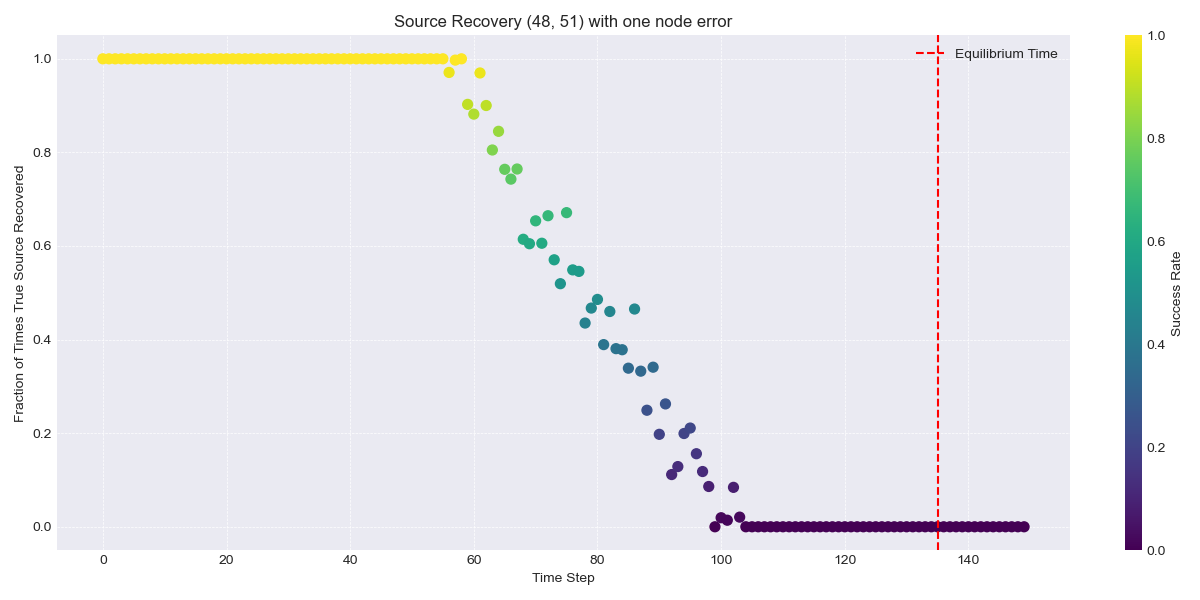
\includegraphics[width=0.9\textwidth]{approx_source_recovery_48_51_Center_of_Mass.png}
\caption{Approximate Source Recovery (48, 51) with Center of Mass Algorithm allowing one-node error}
\label{approx_source_recovery_48_51_Center_of_Mass}
\end{figure}

However, the Center of Mass algorithm's performance near the boundaries remained poor, regardless of whether the grid had wrap-around or fixed boundaries. This is illustrated in Figure \ref{approx_source_recovery_30_70_Center_of_Mass}, where the handling of boundary conditions showed poor performance.

\begin{figure}[H]
\centering
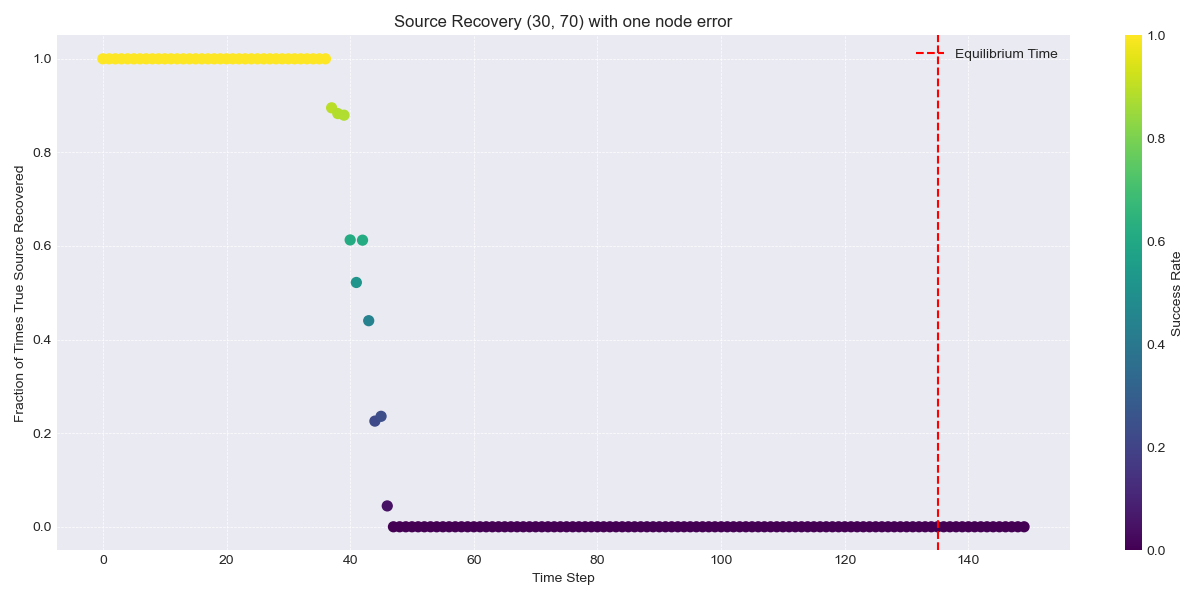
\includegraphics[width=0.9\textwidth]{approx_source_recovery_30_70_Center_of_Mass.png}
\caption{Approximate Source Recovery (30, 70) with Center of Mass Algorithm allowing one-node error}
\label{approx_source_recovery_30_70_Center_of_Mass}
\end{figure}

While the Center of Mass algorithm is computationally efficient, its accuracy is limited, particularly near grid boundaries. By considering a one-node error margin, we can improve the recovery accuracy, but the method still faces challenges in boundary conditions. These findings highlight the importance of adapting source detection algorithms to the specific characteristics and constraints of the grid configuration.\\

Next, we examined the \textbf{Distance Analysis Algorithm}, utilizing Manhattan or Euclidean Distance to identify the source of infection. The algorithm determines the node whose cumulative distance to all infected nodes is minimized. This method, while computationally efficient, suffers from inaccuracies near boundaries.

Initially, the Distance Analysis algorithm demonstrated significant errors in identifying the exact source node. However, when we considered the approximate approach, allowing for a \textit{one-node error margin}, the performance improved markedly. Figure \ref{Source_recovery_distance_analysis} show the results for the central node scenario, indicating better recovery rates with the one-node error margin.

\begin{figure}[H]
\centering
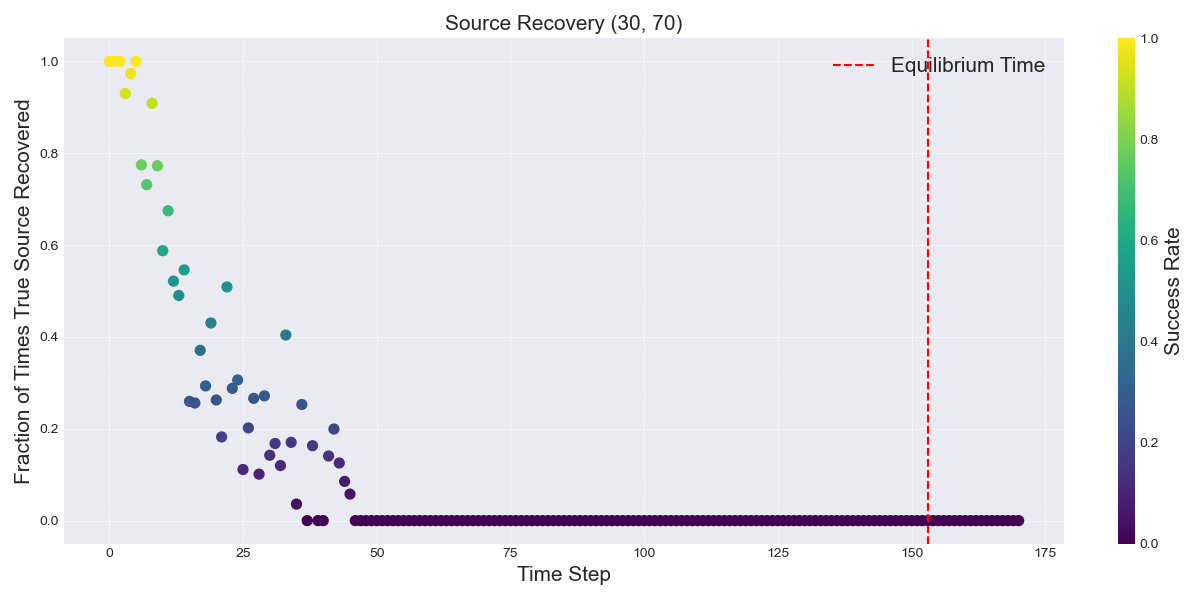
\includegraphics[width=0.49\textwidth]{Source_Recovery_30_70_Distance_analysis.png}
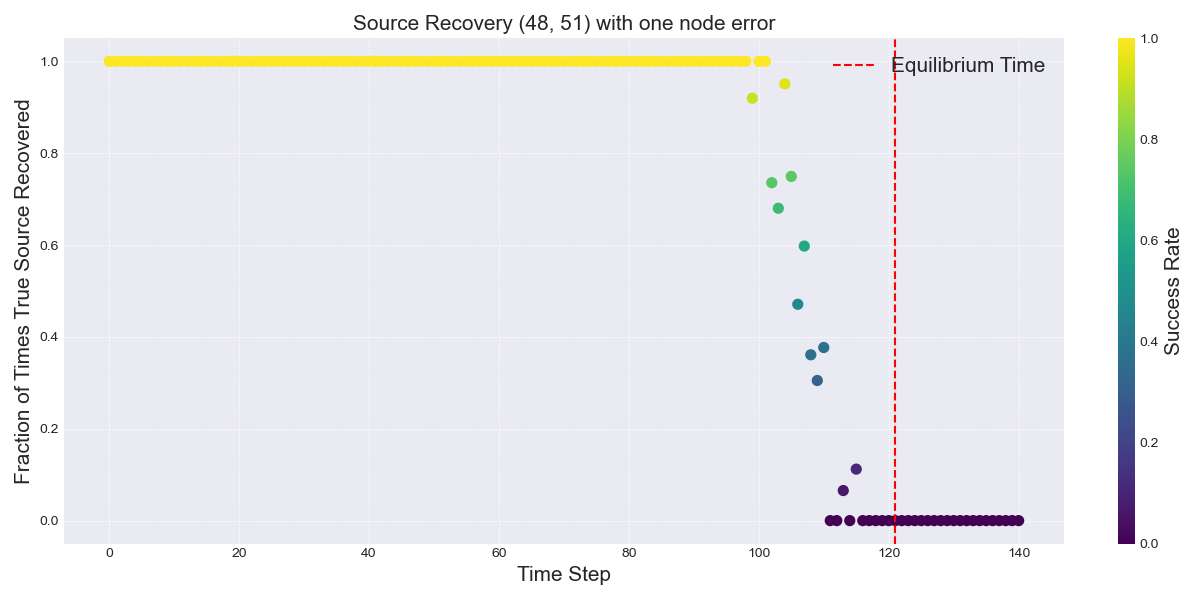
\includegraphics[width=0.49\textwidth]{Approx_Source_Recovery_48_51_Distance_Analysis.png}
\caption{(Left) Source Recovery (30, 70) with Distance Analysis Algorithm without one-node error margin. (Right) Approximate Source Recovery (48, 51) with Distance Analysis Algorithm allowing one-node error}
\label{Source_recovery_distance_analysis}
\end{figure}

In boundary conditions, the Distance Analysis algorithm performed poorly, as illustrated in Figure \ref{boundary_handling_distance_analysis}. The accuracy significantly drops when the infection reaches the boundaries, indicating a loss of critical information for source detection.

\begin{figure}[H]
\centering
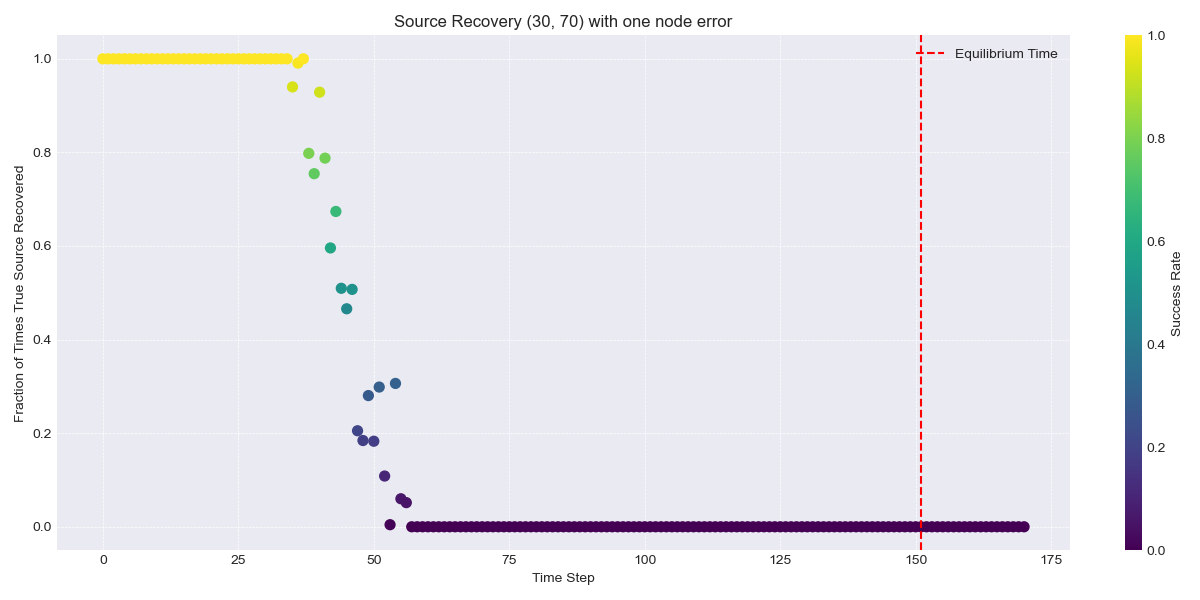
\includegraphics[width=0.9\textwidth]{Approx_Source_Recovery_30_70_Distance_Analysis.png}
\caption{Approximate Source Recovery (30, 70) with Distance Analysis Algorithm allowing one-node error}
\label{boundary_handling_distance_analysis}
\end{figure}

Upon comparing the three algorithms, the Jordan Center algorithm consistently demonstrated the highest accuracy in source detection, particularly in wrap-around grid configurations. This can be attributed to its ability to handle uniform connectivity across the grid, which is not affected by boundary conditions. The Center of Mass and the Distance Analysis algorithms, while computationally efficient, showed limitations in accuracy, especially near grid boundaries. The one-node error margin approach significantly improved their performances, making them a viable option for quick approximations.\\

In summary, the grid-based algorithms implemented in this study provided valuable insights into the effectiveness of different approaches for source detection in epidemiological models. The Jordan Center algorithm emerged as the most accurate, especially in wrap-around grid configurations, making it suitable for both grid-based and complex network models. The Center of Mass and Distance Analysis algorithms, while less accurate, offered computational efficiency and improved performance with the one-node error margin approach.\\

Moving forward, we will explore the application of these algorithms to complex network models to further enhance our understanding of disease spread dynamics and improve the traceability of infection sources.

\subsection{Centrality Measures in Complex Network Models}

We move on now to complex network models, which are crucial for a comprehensive understanding of disease spread dynamics in real-world scenarios. Unlike grid-based models, complex networks exhibit diverse structures and connectivity patterns that significantly influence the spread of infections. We used several types of complex networks, including Erdős–Rényi graphs, Random Regular graphs, and Random Geometric graphs. These network types are illustrated in Figure \ref{fig:network_types}.

\begin{figure}[H]
    \centering
    \begin{subfigure}{0.33\textwidth}
        \centering
        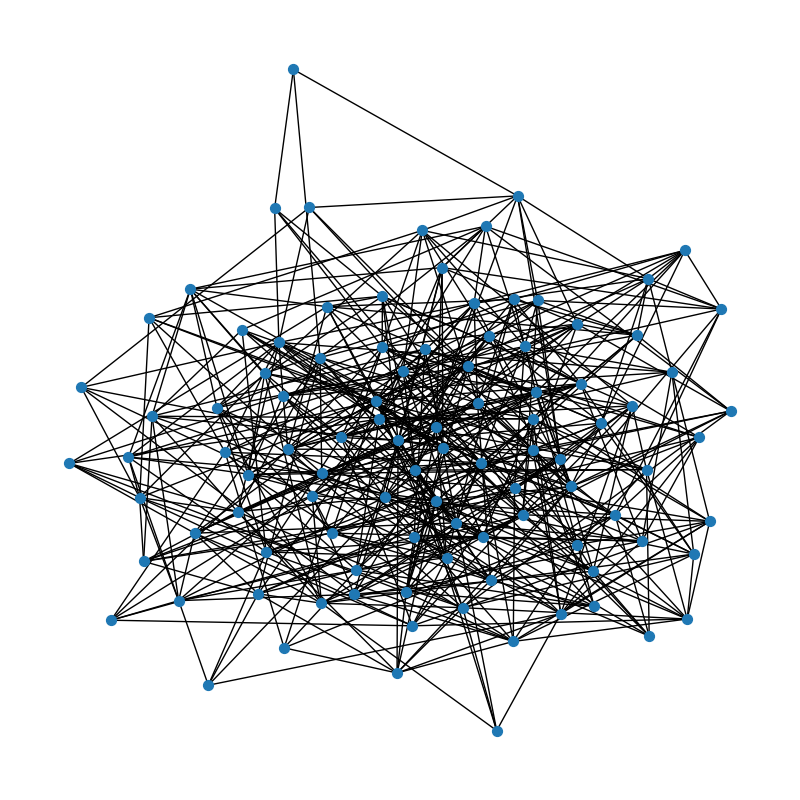
\includegraphics[width=\textwidth]{erdos_renyi_graph.png}
        \caption{Erdős–Rényi Graph}
        \label{fig:erdos_renyi_graph}
    \end{subfigure}
    \begin{subfigure}{0.33\textwidth}
        \centering
        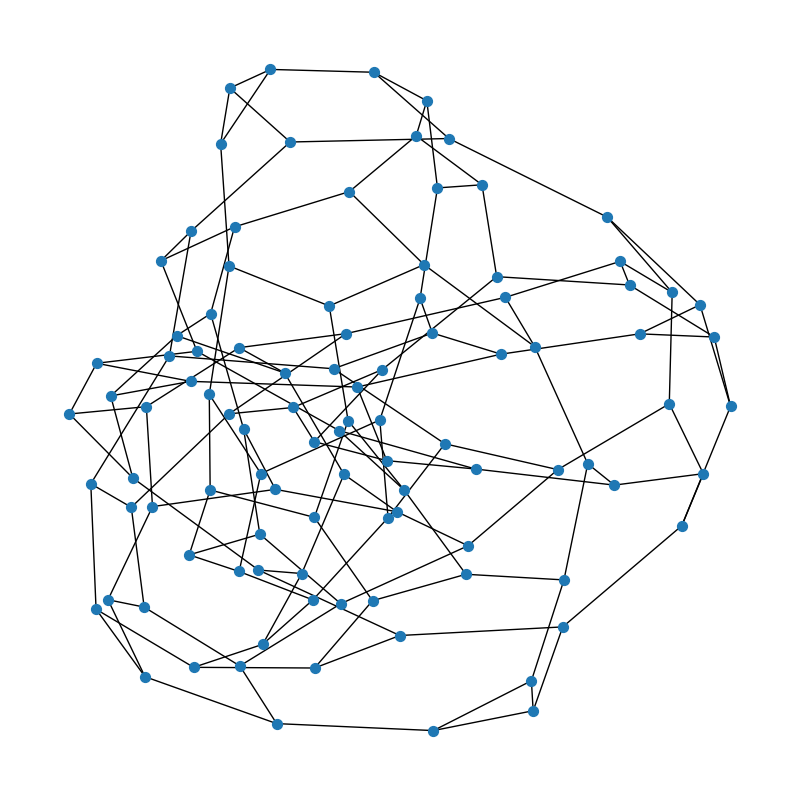
\includegraphics[width=\textwidth]{random_regular_graph.png}
        \caption{Random Regular Graph}
        \label{fig:random_regular_graph}
    \end{subfigure}
    \begin{subfigure}{0.33\textwidth}
        \centering
        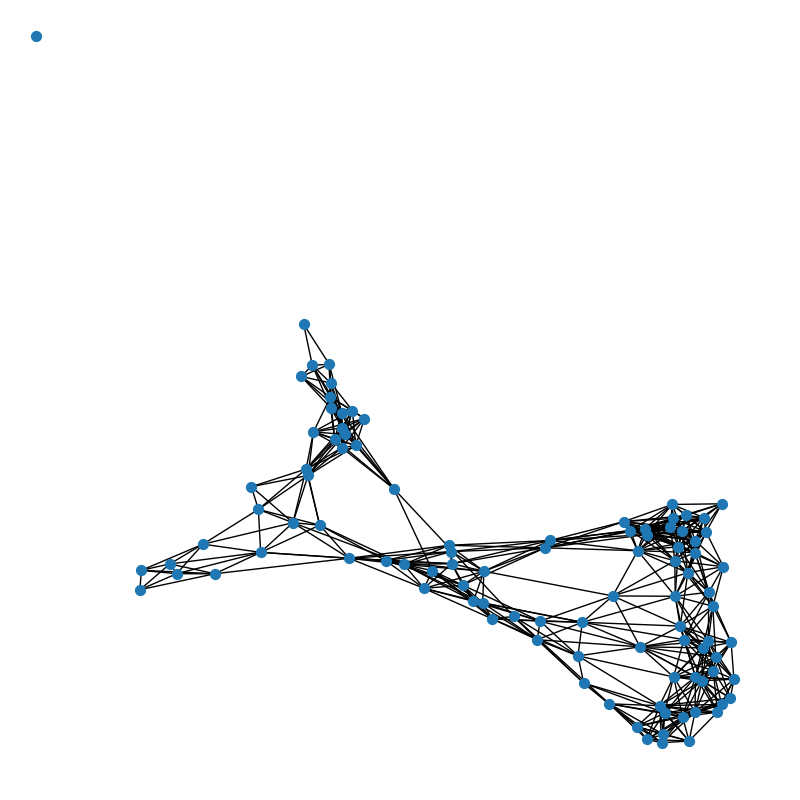
\includegraphics[width=\textwidth]{random_geometric_graph.png}
        \caption{Random Geometric Graph}
        \label{fig:random_geometric_graph}
    \end{subfigure}
    \caption{Examples of Complex Network Structures}
    \label{fig:network_types}
\end{figure}

We chose these networks due to their varying structural properties. Erdős–Rényi graphs are simple random graphs where each edge is included with a fixed probability. Random Regular graphs have a fixed degree for each node, ensuring uniform connectivity. Random Geometric graphs represent spatial networks where nodes are connected if they are within a certain distance, introducing heterogeneity in node degrees.\\

To enhance source detection in these complex networks, we employed various centrality measures \cite{jiang2017}:
\label{centrality_measure}
\begin{enumerate}
    \item \textbf{Eccentricity + Closeness Centrality:} This combined measure uses both eccentricity and closeness scores to identify central nodes. 
    \item \textbf{Eccentricity:} Defined as the greatest distance between a node and any other node in the network, used to find the "central" node \cite{newman2010}.
    \item \textbf{Betweenness Centrality:} Measures the extent to which a node lies on the shortest paths between other nodes, highlighting nodes critical for the flow of infection \cite{girvan2002}.
    \item \textbf{Eigenvector Centrality:} Assigns relative scores to all nodes based on the principle that connections to high-scoring nodes contribute more to a node's score.
    \item \textbf{Closeness Centrality:} Measures the average length of the shortest path from a node to all other nodes in the network, indicating how quickly information spreads from a given node to others.
\end{enumerate}

The implementation of these centrality measures was integrated into the network simulation, and their performance was tested on various network structures. The evaluation criteria included accuracy and time complexity under varying network conditions and infection parameters.\\

Figure \ref{fig:centrality_measures_explained} from Jiang et al. \cite{jiang2017} provides a comprehensive illustration of these centrality measures.

\begin{figure}[H]
    \centering
    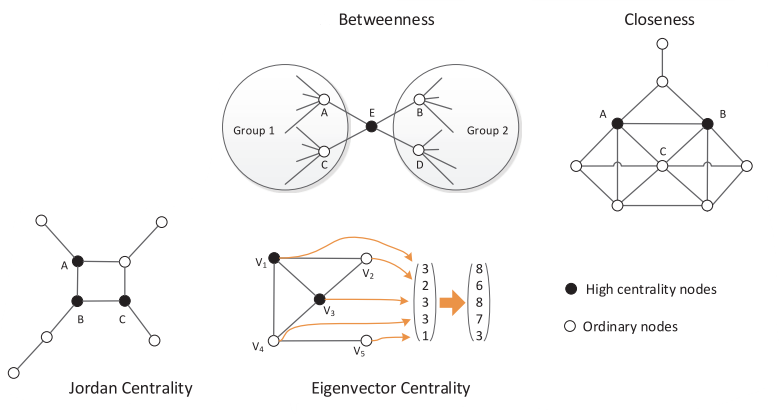
\includegraphics[width=0.9\textwidth]{centrality_measures.png}
    \caption{Centrality Measures Explained (Jiang et al., 2017)}
    \label{fig:centrality_measures_explained}
\end{figure}

In this figure, different centrality measures are visually explained:
\begin{itemize}
    \item \textbf{Betweenness:} Nodes that frequently appear on shortest paths between other nodes.
    \item \textbf{Closeness:} Nodes that can reach other nodes most quickly.
    \item \textbf{Jordan:} Nodes that minimize the maximum distance to other nodes.
    \item \textbf{Eigenvector:} Nodes that are connected to other well-connected nodes.
\end{itemize}

These centrality measures offer different insights into network structure and dynamics, aiding in the accurate identification of infection sources. The implementation of these centrality measures was integrated into the network simulation, and their performance was tested on various network structures. The evaluation criteria included accuracy and computational efficiency under varying network conditions and infection parameters \cite{liu2011}. Their performance is further analyzed in the subsequent sections.\\

First, let us delve into the accuracy of these centrality measures. Figure \ref{fig:accuracy_centrality_measures} shows the accuracy of various centrality measures on different network types. We executed each of the source detection algorithms 400 times across various stages of the infection and different graph configurations to generate this plot.

\begin{figure}[H]
    \centering
    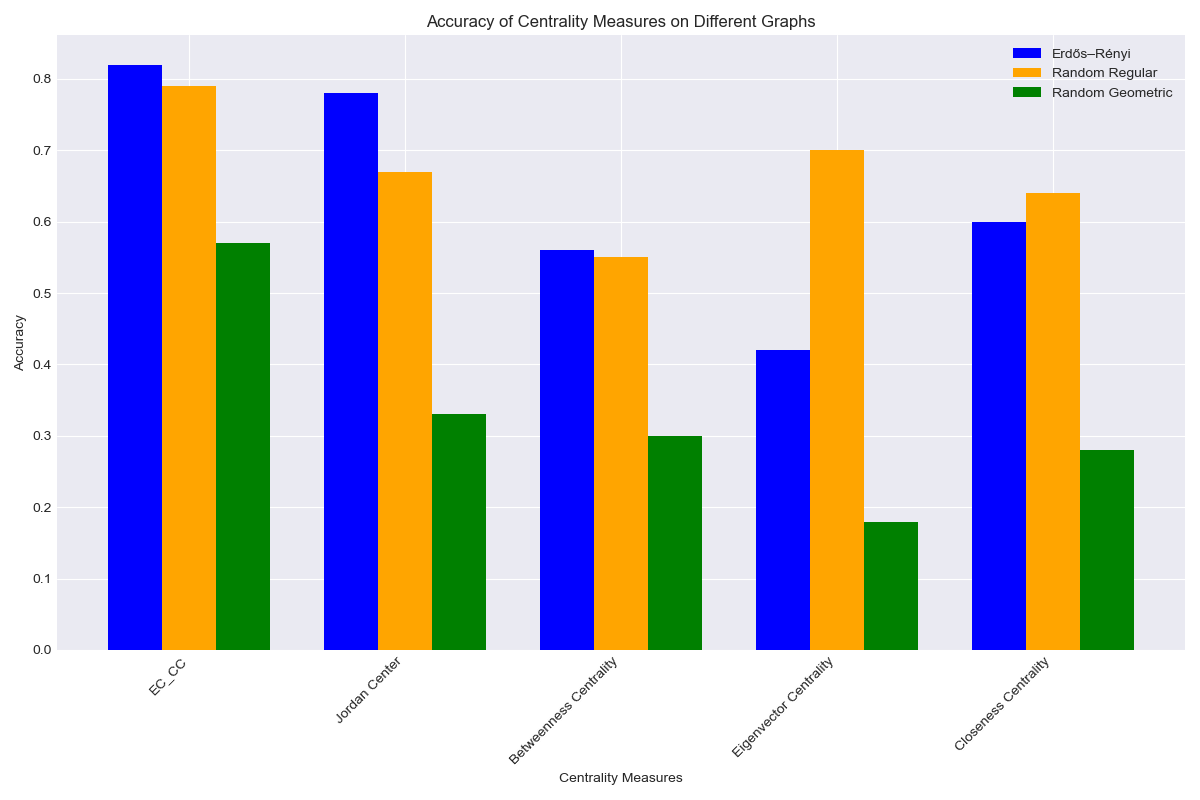
\includegraphics[width=0.9\textwidth]{Accuracy_Centrality_Measures.png}
    \caption{Accuracy of Centrality Measures on Different Graphs}
    \label{fig:accuracy_centrality_measures}
\end{figure}

From the accuracy plot, we observe that the combination of Eccentricity and Closeness Centrality (EC\_CC) consistently demonstrates the highest accuracy across all network types. This is likely because Eccentricity identifies the node that minimizes the maximum distance to all other nodes, while Closeness Centrality ensures that the node is centrally located in terms of average shortest path distances. Together, they provide a robust indication of the central node, which is often the source of the infection.\\

For Erdős–Rényi and Random Regular graphs, the accuracy is relatively high. This can be attributed to the regularity and homogeneity of these graphs, where nodes tend to have similar numbers of neighbors, allowing centrality measures to perform effectively. The consistent connectivity patterns in these graphs make it easier for the algorithms to identify the central nodes accurately.

In contrast, the accuracy is lower for Random Geometric graphs. These graphs have irregular structures, with varying node degrees and connectivity patterns, especially near the boundaries. The irregularities and the presence of boundary nodes, which have fewer neighbors, make it challenging for centrality measures to accurately identify the infection source. The varying density and proximity-based connections disrupt the uniformity, leading to lower accuracy in source detection.\\

However, accuracy is not the only criterion to consider. The computational efficiency of these algorithms is equally important, especially for large-scale networks. Figure \ref{fig:average_time_centrality_measures} illustrates the average time taken by various centrality measures on different network types.

\begin{figure}[H]
    \centering
    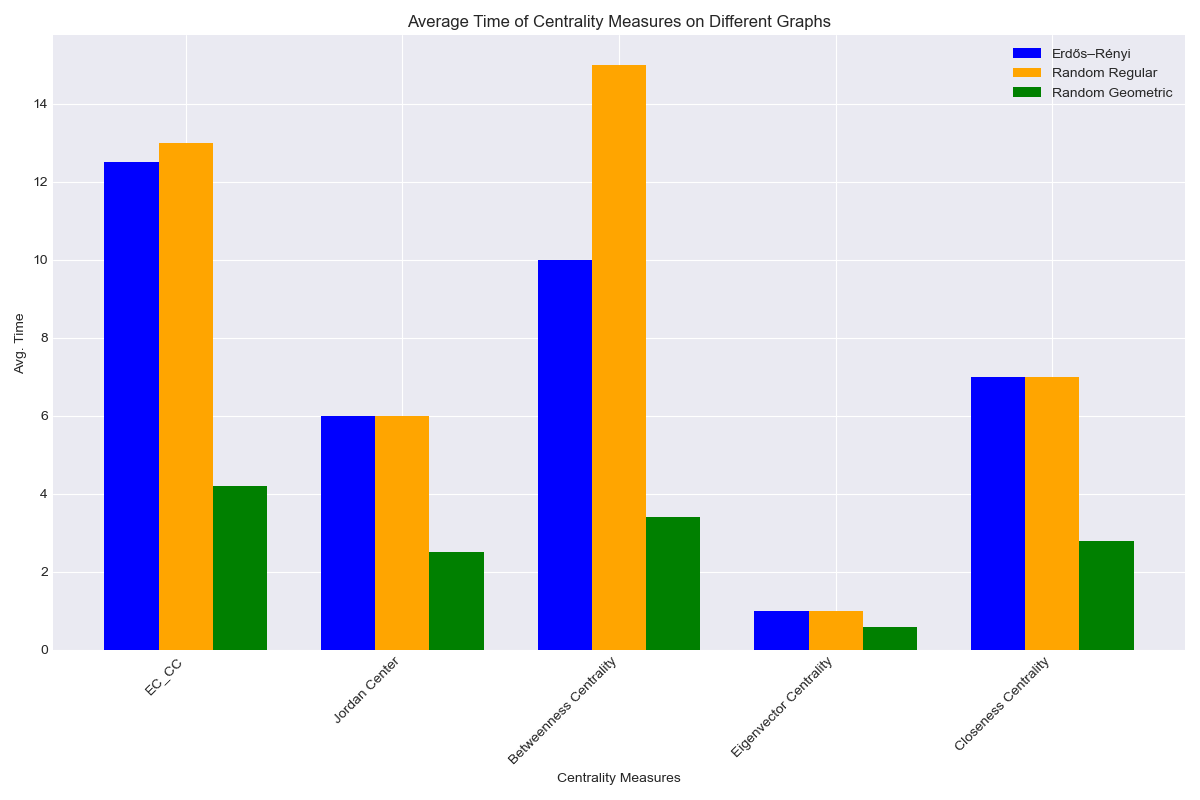
\includegraphics[width=0.9\textwidth]{Average_Time_Centrality_Measures.png}
    \caption{Average Time of Centrality Measures on Different Graphs}
    \label{fig:average_time_centrality_measures}
\end{figure}

The combination of Eccentricity and Closeness Centrality (EC\_CC), while accurate, is the most time-consuming. This is because these measures involve complex calculations that consider the distances between all pairs of nodes. The high time complexity can be a significant drawback in large networks where quick decision-making is crucial.

Betweenness Centrality also takes a considerable amount of time due to its dependency on the shortest paths between all node pairs. It provides valuable insights into the network's flow structure but at the cost of computational efficiency.

Eigenvector Centrality is relatively fast but sacrifices accuracy, particularly in irregular networks. It assigns scores based on the principle that connections to high-scoring nodes contribute more to a node's score. While this is useful in some contexts, it may not always accurately identify the infection source, especially in heterogeneous networks.

Closeness Centrality strikes a balance between time and accuracy, performing well across different network types. It measures the average length of the shortest path from a node to all other nodes, providing a good indication of centrality without the computational overhead of Betweenness or EC\_CC.

Jordan Centrality provides a favorable balance between accuracy and time complexity, making it an excellent choice for source detection algorithms. It performs effectively on both grid-based and network-based models.\\

In summary, the choice of centrality measure depends on the specific requirements of the analysis. For high accuracy, especially in regular networks, EC\_CC is preferred despite its higher computational cost. For faster computations, Eigenvector or Closeness Centrality might be more suitable, particularly in large or irregular networks.\\

The results from our study highlight the strengths and weaknesses of various centrality measures for source detection in complex networks. By understanding these trade-offs, we can select the most appropriate algorithm based on the network structure and the specific requirements of the task at hand.



\section{Stochastic Approach}

Given that our models already incorporate stochasticity through probabilistic spreading, we explored an additional route to simulate infection spread: the stochastic approach model. This approach differs from our current models, which advance one step at a time using timestamps. Instead, the stochastic approach uses continuous-time Markov processes to simulate the timing of infection events, providing a more nuanced understanding of disease dynamics and allowing for real-time simulations.

We implemented this new stochastic model using the Gillespie Algorithm, which is suitable for simulating systems with random events such as disease spread. The Gillespie Algorithm allows us to model the discrete nature of infection events and the inherent randomness in the timing of these events. The infection times follow an exponential distribution, capturing the stochastic nature of real-world scenarios. The mathematical foundation of the stochastic approach involves Stochastic Differential Equations (SDEs) for the SIRS model, which incorporate Wiener processes to account for random perturbations in the state of susceptible, infected, and recovered individuals. This allows for the incorporation of random fluctuations and noise into the infection dynamics \cite{liu2020, paladini2011, rodriguez2020}.

The flowchart of the Gillespie Algorithm is shown in Figure \ref{fig:gillespie_algorithm}.

\begin{figure}[H]
    \centering
    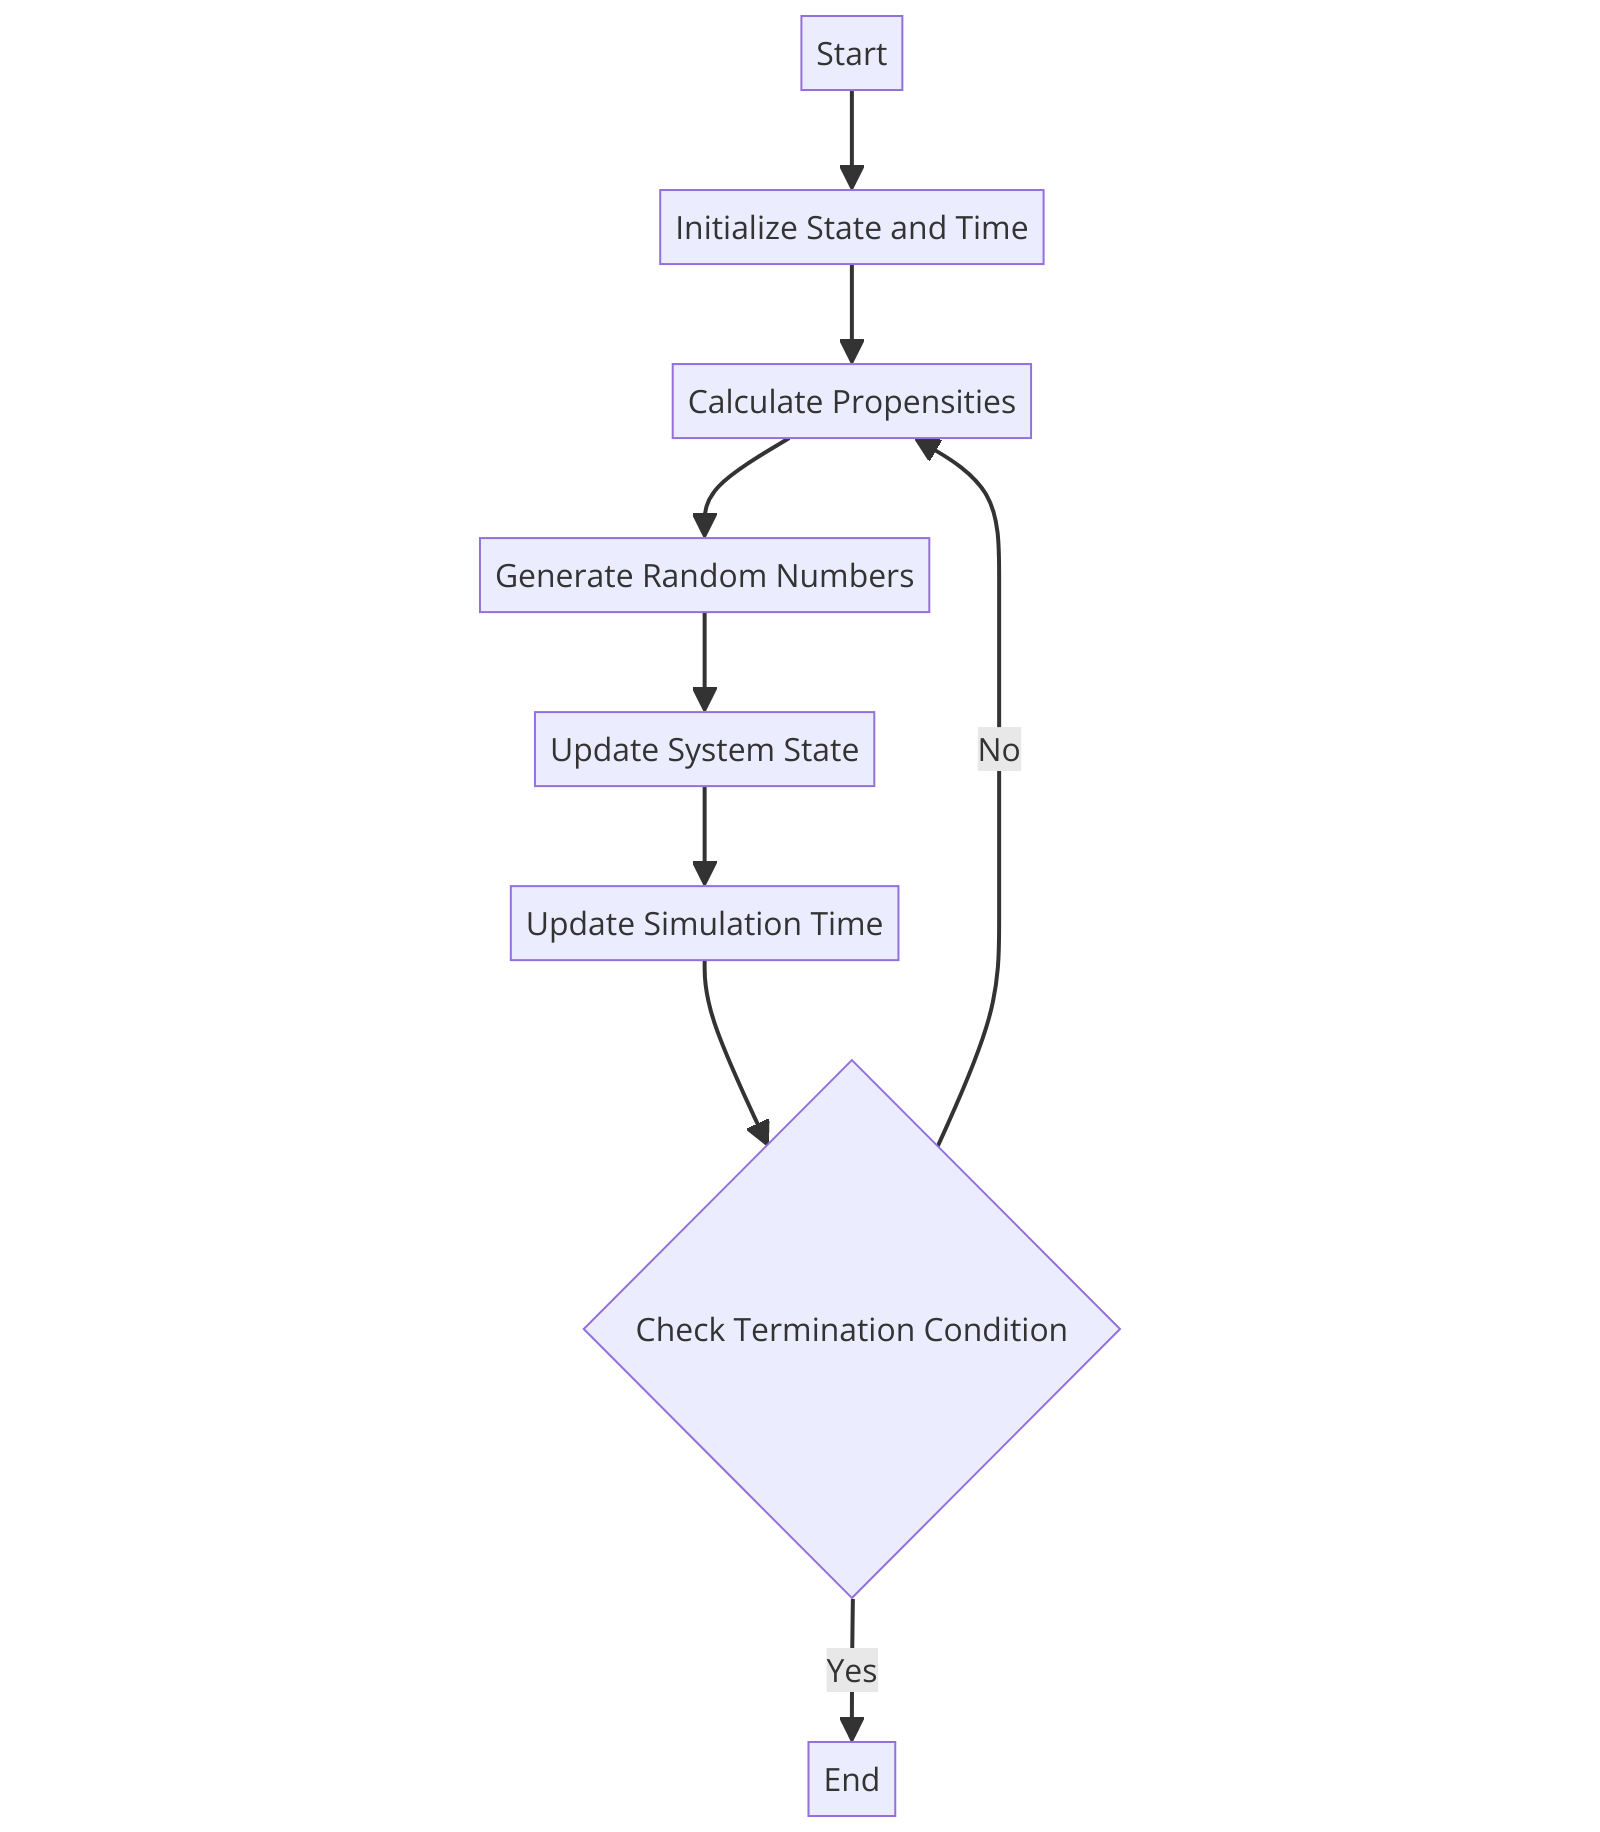
\includegraphics[width=0.9\textwidth]{flowchart_algorithm.png}
    \caption{Flowchart of the Gillespie Algorithm}
    \label{fig:gillespie_algorithm}
\end{figure}

By incorporating stochastic elements, we can capture the unpredictable fluctuations that occur in real-world disease spread scenarios. This randomness affects the performance of source detection algorithms, as the spread patterns are less predictable and more diverse \cite{britton2010, keeling2008}.

We performed a comparative analysis between our probabilistic spreading models and the new stochastic approach to highlight the differences and advantages. The stochastic models provide a more realistic simulation of infection dynamics, accounting for the inherent uncertainties in real-world scenarios \cite{allen2017, ball2016}.

The comparison of the probabilistic and stochastic models is illustrated in Figure \ref{fig:Comparison_Probabilistic_Stochastic}.

\begin{figure}[H]
    \centering
    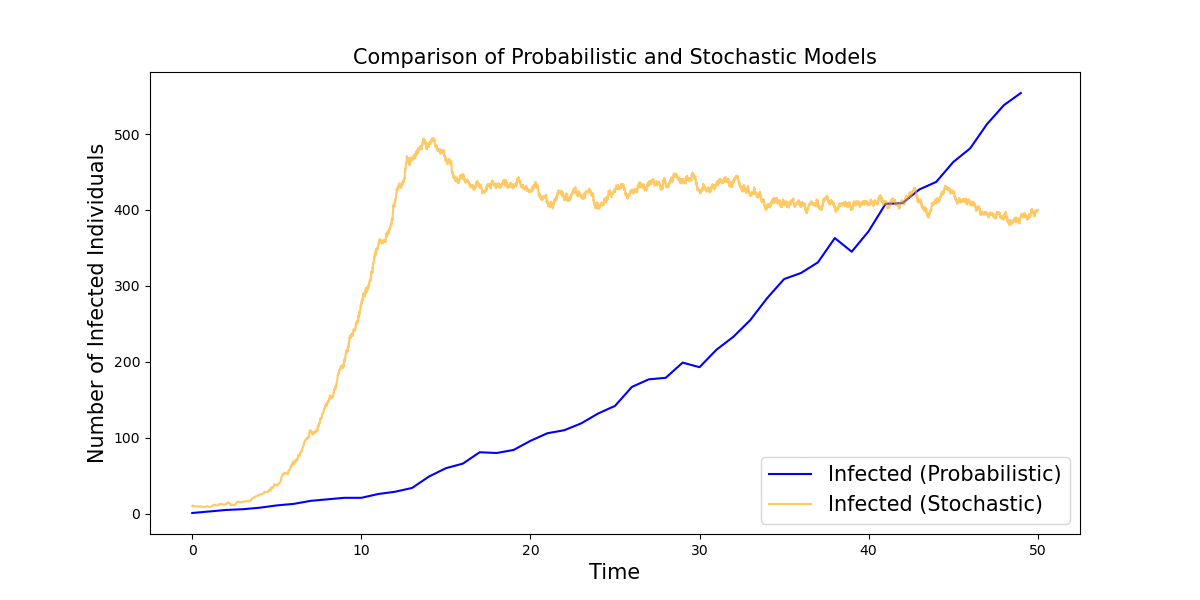
\includegraphics[width=0.9\textwidth]{Comparison_Probabilistic_Stochastic Models.png}
    \caption{Comparison of Probabilistic and Stochastic Models}
    \label{fig:Comparison_Probabilistic_Stochastic}
\end{figure}

From Figure \ref{fig:Comparison_Probabilistic_Stochastic}, several key differences and observations can be made:

\begin{itemize}
    \item \textbf{Variability and Noise:} The stochastic model (orange line) shows significant variability and noise, capturing the random fluctuations in the number of infected individuals. This is consistent with real-world scenarios where infection dynamics are influenced by numerous unpredictable factors. The probabilistic model (blue line) shows a smoother trajectory, representing the average behavior of the infection spread over discrete time steps.
    
    \item \textbf{Peak Infection:} The stochastic model reaches a higher peak of infection more quickly, reflecting the potential for rapid outbreaks due to random events. The probabilistic model shows a more gradual increase in infections, highlighting the average spread without accounting for sudden changes.
    
    \item \textbf{Equilibrium State:} Both models eventually reach an equilibrium state, but the stochastic model's equilibrium fluctuates more due to ongoing random events. The probabilistic model's equilibrium is more stable, reflecting the average steady-state behavior.
\end{itemize}

\subsubsection{Advantages of the Stochastic Approach:}

\begin{itemize}
\item Captures the randomness and variability observed in real-world infection spread, which deterministic models may overlook.
\item Provides a more nuanced understanding of disease dynamics by accounting for random fluctuations and noise.
\item Leads to more robust and reliable predictions of disease spread and source detection, better reflecting the inherent uncertainties in real-world scenarios \cite{hethcote2000}.
\item Allows for real-time simulations, making it suitable for dynamic and rapidly changing epidemic scenarios.
\end{itemize}

In summary, incorporating stochastic elements into infection spread models significantly enhances their realism and reliability. The stochastic models account for the inherent randomness and noise present in real-world disease spread, leading to more accurate and robust predictions. This comparative analysis underscores the importance of stochastic modeling in epidemiological research and the need for further development of these models to better understand and control disease spread \cite{ross2011}.

\section{Conclusion}

This chapter has detailed the design and implementation of grid-based and complex network models for simulating infectious disease spread. By employing various source detection algorithms and centrality measures, we aimed to improve the traceability of infection sources. The integration of stochastic elements further enhanced the realism of our simulations, providing a comprehensive framework for understanding disease dynamics.

The Jordan Center algorithm demonstrated high accuracy in wrap-around grid configurations but showed limitations in fixed boundary scenarios. Centrality measures like EC\_CC proved to be the most effective for source detection in complex networks, although at the cost of higher computational time.\\

In summary, our findings highlight the importance of selecting appropriate algorithms and centrality measures based on the network structure and the specific requirements of the analysis. The choice of algorithm significantly impacts the accuracy and computational efficiency of source detection in epidemiological models.